\documentclass[9pt]{beamer}

\input{MainTop.tex}


\usepackage{algpseudocode}

% \title{C - Big Data Analysis}
\title[]{An Experimental Study of Memory Management in Rust Programming for Big Data Processing}
% \subtitle{Gradient Descent}
% \date{\today}
\date{May, 2020}
\author[Shinsaku Okazaki]{Shinsaku Okazaki}
\institute{Boston University}
% \institute{}

\begin{document}

\maketitle

% \setbeamertemplate{itemize items}[triangle]

\setbeamertemplate{itemize item}{\color{red}$\triangleright$}
\setbeamertemplate{itemize subitem}{\color{blue}$\triangleright$}



% \begin{frame}{Table of contents}
%   \setbeamertemplate{section in toc}[sections numbered]
%  \tableofcontents[hideallsubsections]
% \end{frame}


%%%%%%%%%%%%%%%%%%%%%%%%%%%%%%%%%%%%%%%%%%%%
%%%%%%%%%%%%%%%%%%%%%%%%%%%%%%%%%%%%%%%%%%%%

\begin{frame}[fragile]{Motivation}

Development of modern Big Data processing tools has some problems!

\begin{itemize}

  \item \textcolor{blue}{Generative Garbage Collection}
  \item \textcolor{blue}{Stop-The-World}
  \item \textcolor{blue}{Memory Safe impelementation}
\end{itemize}

\textcolor{blue}{Rust} can be a ideal candidate for development of Big Data processing tools.



\end{frame}


%%%%%%%%%%%%%%%%%%%%%%%%%%%%%%%%%%%%%%%%%%%%
%%%%%%%%%%%%%%%%%%%%%%%%%%%%%%%%%%%%%%%%%%%%

\begin{frame}[t, fragile]{Rust}

    \textcolor{blue}{Rust} is a system language which has unique memory management concept.

    \begin{itemize}
        \item \blueb{A system language does not have Garbage Collection.}
        \item \blueb{Rust ensures memory safety.}
        \item \blueb{It is easy to write safe multithreading code in Rust.}
    \end{itemize}
\end{frame}

%%%%%%%%%%%%%%%%%%%%%%%%%%%%%%%%%%%%%%%%%%%%
%%%%%%%%%%%%%%%%%%%%%%%%%%%%%%%%%%%%%%%%%%%%

\begin{frame}[fragile]{Problem Description}


    Do following concepts have impact on runtime performance of algorithms?
    \begin{itemize}
        \item \blueb{Complex object}
        \item \blueb{Different  variable  types}
        \item \blueb{Reference Count}
        \item \blueb{Multithreading}
        \item \blueb{Common Big Data algorithms}
    \end{itemize}
\end{frame}

%%%%%%%%%%%%%%%%%%%%%%%%%%%%%%%%%%%%%%%%%%%%
%%%%%%%%%%%%%%%%%%%%%%%%%%%%%%%%%%%%%%%%%%%%

\begin{frame}[fragile]{Complex Object}

    In Big Data processing, data is represented by complex objects.

    \begin{minipage}[t]{0.2\linewidth}\centering
        \begin{lstlisting}
            struct CustomerOwned {
                key: i32,
                age: i32,
                num_purchase: i32,
                total_purchase: f64,
                duration_spent: f64,
                duration_since: f64,
                zip_code: String,
                address: String,
                country: String,
                state: String,
                first_name: String,
                last_name: String,
                province: String,
                comment: String,
                order: OrderOwned
            }
        \end{lstlisting}
    \end{minipage}\hfill

\end{frame}
%%%%%%%%%%%%%%%%%%%%%%%%%%%%%%%%%%%%%%%%%%%%
%%%%%%%%%%%%%%%%%%%%%%%%%%%%%%%%%%%%%%%%%%%%

\begin{frame}[t, fragile]{Different Variable Types}

    Each one has \textcolor{blue}{different memory representation.}
    \begin{itemize}
        \item \blueb{Owner}
        \item \blueb{Reference}
        \item \blueb{Slice}
    \end{itemize}

    Each one may have \textcolor{blue}{different memory access time.}

\pause


Text



\end{frame}

%%%%%%%%%%%%%%%%%%%%%%%%%%%%%%%%%%%%%%%%%%%%
%%%%%%%%%%%%%%%%%%%%%%%%%%%%%%%%%%%%%%%%%%%%

\begin{frame}[fragile]{Reference Counting}

    Advantage
    \begin{itemize}
        \item \blueb{Sharing ownership}
        \item \blueb{Dinamic memory de/allocation}
    \end{itemize}

    Disadvantage
    \begin{itemize}
        \item \blue{Need to check reference count}
        \item \blue{Heap allocation}
    \end{itemize}


\end{frame}

%%%%%%%%%%%%%%%%%%%%%%%%%%%%%%%%%%%%%%%%%%%%
%%%%%%%%%%%%%%%%%%%%%%%%%%%%%%%%%%%%%%%%%%%%

\begin{frame}[fragile]{Multithreading}
    Atomic Reference Counting


    Advantage
    \begin{itemize}
        \item \blueb{Sharing ownership}
        \item \blueb{Dinamic memory de/allocation}
        \item \blueb{Sharing among multithreads}

    \end{itemize}

    Disadvantage
    \begin{itemize}
        \item \blueb{Need to check reference count}
        \item \blueb{Heap allocation}
        \item \blueb{Atomic operation}
    \end{itemize}

\end{frame}

%%%%%%%%%%%%%%%%%%%%%%%%%%%%%%%%%%%%%%%%%%%%
%%%%%%%%%%%%%%%%%%%%%%%%%%%%%%%%%%%%%%%%%%%%

\begin{frame}[fragile]{Common Big Data algorithms}

    \begin{itemize}
        \item \blueb{Merge-sort}
        \item \blueb{Tree-aggtegate}
        \item \blueb{K-Nearest-Neighbors (KNN)}
    \end{itemize}

\end{frame}

%%%%%%%%%%%%%%%%%%%%%%%%%%%%%%%%%%%%%%%%%%%%
%%%%%%%%%%%%%%%%%%%%%%%%%%%%%%%%%%%%%%%%%%%%

\begin{frame}[fragile]{Experiment 1: Accessing Object with Different Variable Type}

    Question
    \begin{itemize}
        \item How much are memory access times different among different variable types used in complex objects?
    \end{itemize}

    Evaluation
    \begin{itemize}
        \item \blueb{Custruct complext objects}
        \item With different variable types: \blueb{Owner, Reference, Slice}
        \item Measure time to \blueb{access to fields of complex objects}
    \end{itemize}

\end{frame}

%%%%%%%%%%%%%%%%%%%%%%%%%%%%%%%%%%%%%%%%%%%%
%%%%%%%%%%%%%%%%%%%%%%%%%%%%%%%%%%%%%%%%%%%%

\begin{frame}[fragile]{Experiment 1: Accessing Object with Different Variable Type}

    \begin{figure}[hp]
        \centering
        \begin{center}
                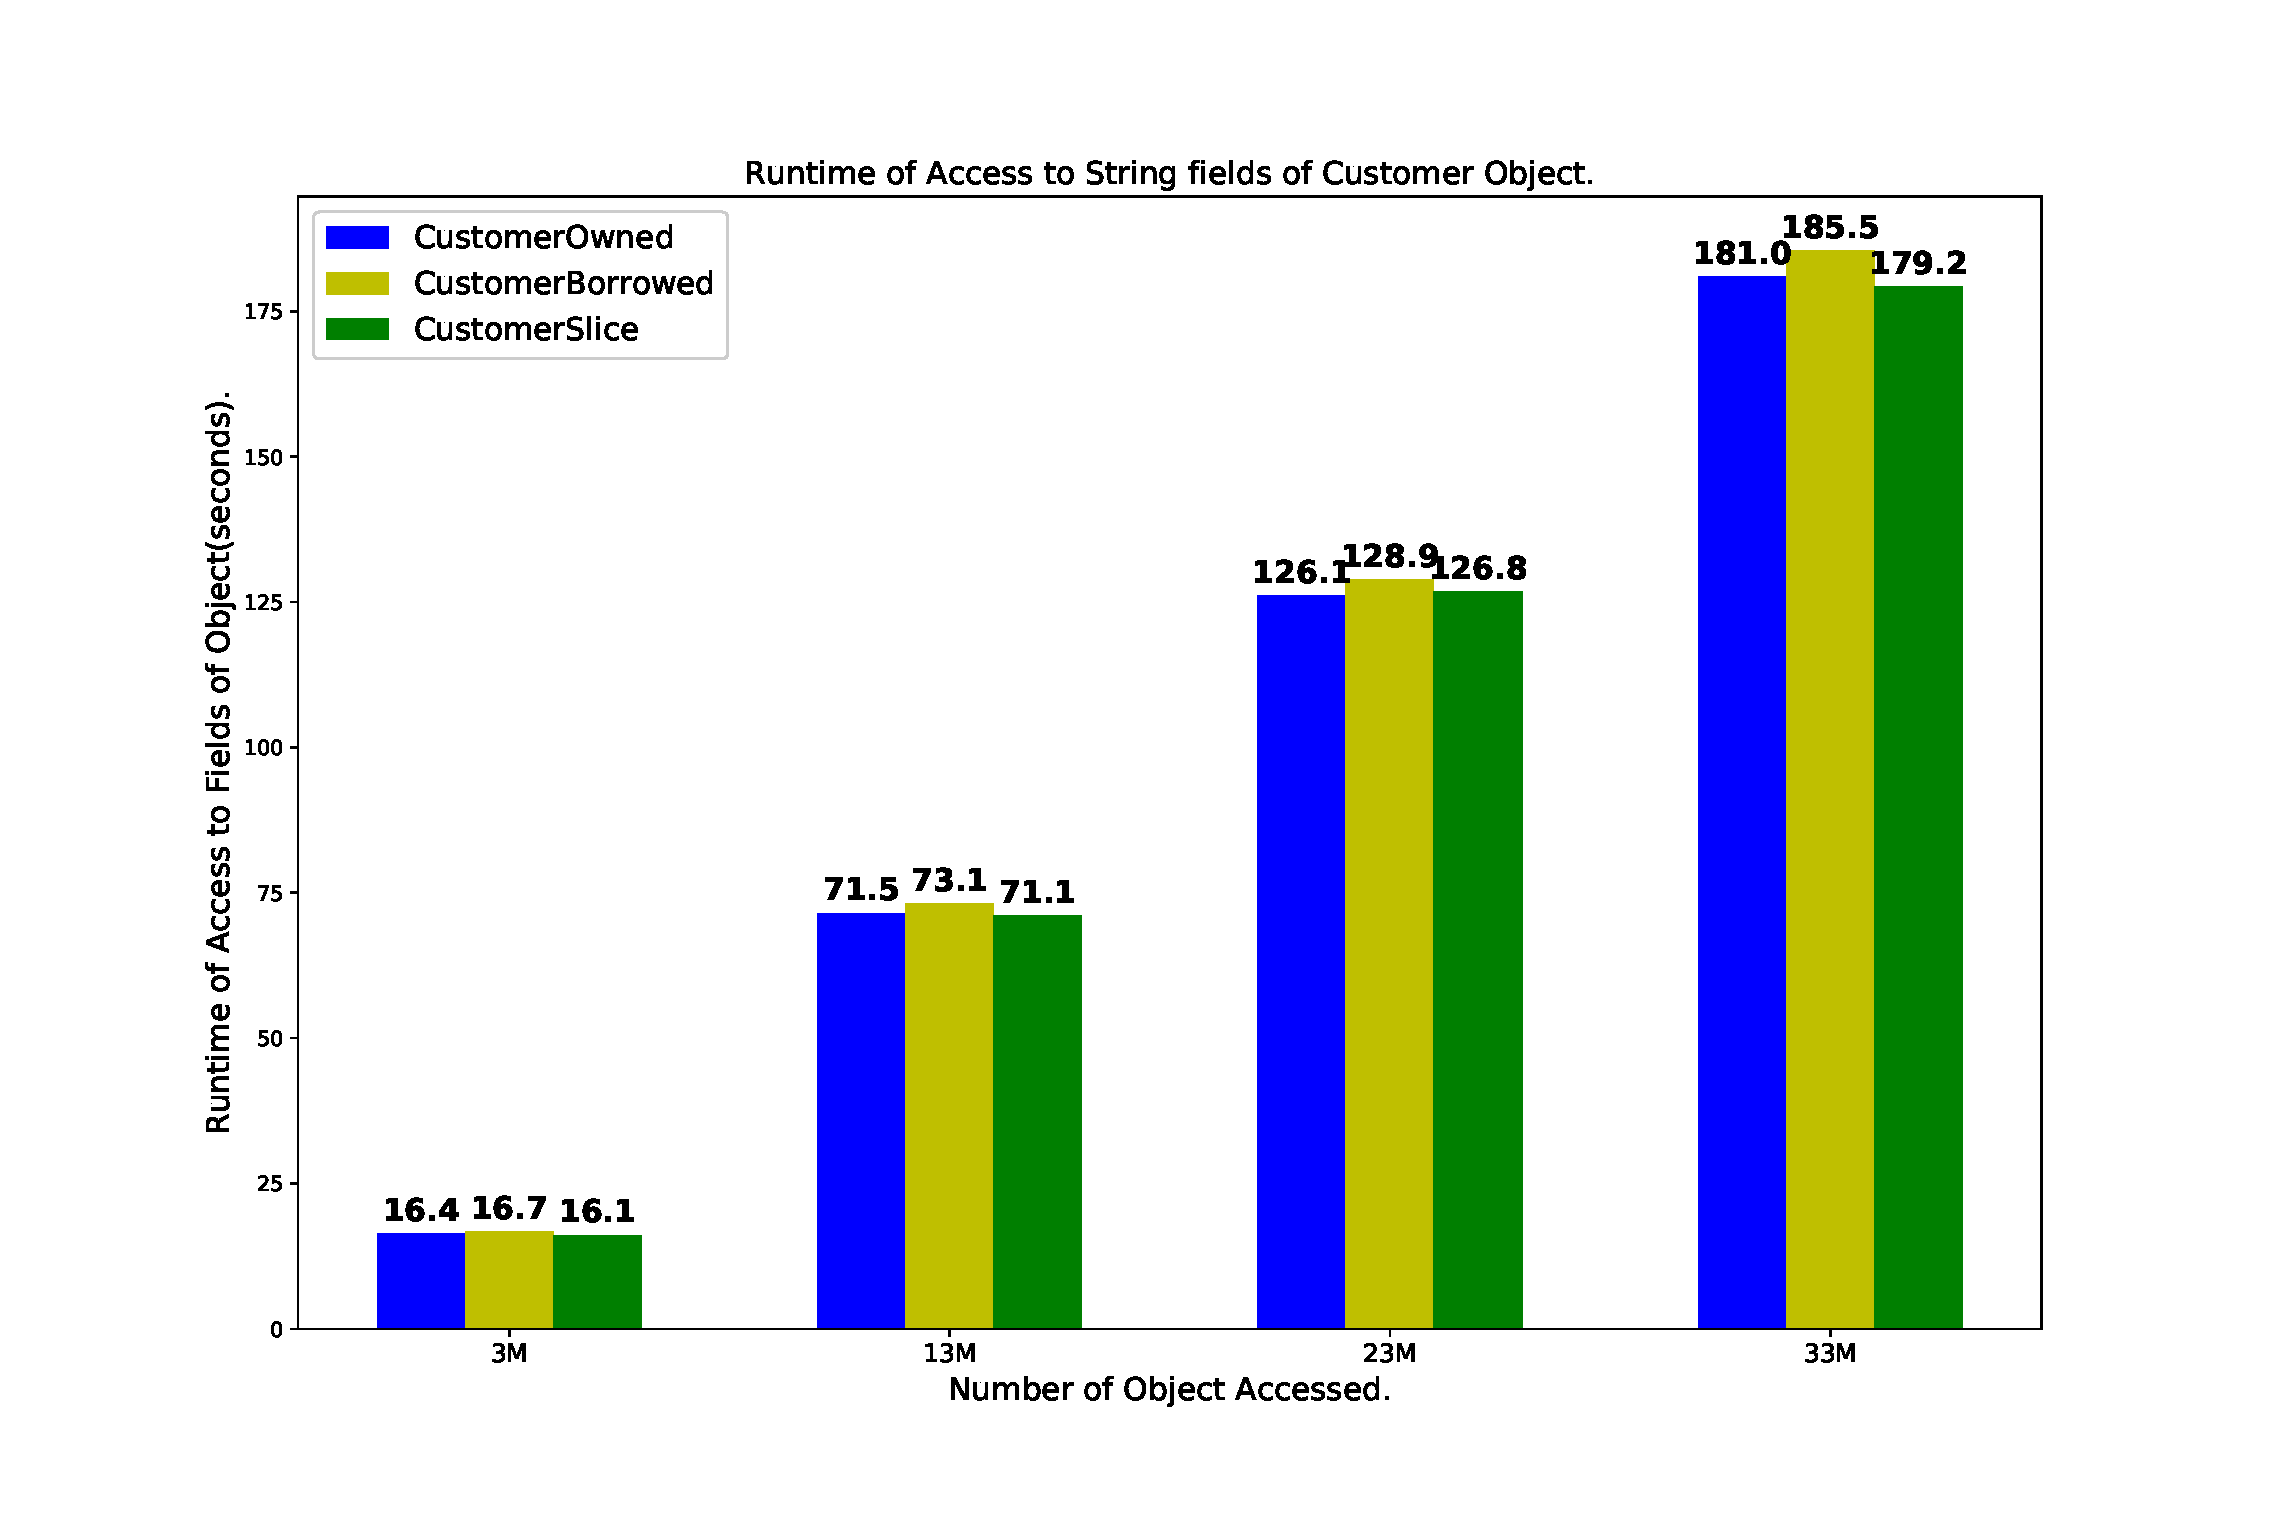
\includegraphics[width=1\textwidth]{images/rust_access_different_poniter_init.eps}
                \captionsetup{labelformat=empty}
                % \caption{\textbf{}}
        \end{center}
    \end{figure}
\end{frame}

%%%%%%%%%%%%%%%%%%%%%%%%%%%%%%%%%%%%%%%%%%%%
%%%%%%%%%%%%%%%%%%%%%%%%%%%%%%%%%%%%%%%%%%%%

\begin{frame}[fragile]{Experiment 2: Assessment of different reference methods in Rust}

    Question
    \begin{itemize}
        \item How much does Reference Counting slowdown time for dropping its variable?
    \end{itemize}

    Evaluation
    \begin{itemize}
        \item \blueb{Custruct complext objects}
        \item \blueb{Reference Counting} vs \blueb{reference}
        \item Measure time to \blueb{drop variables of complex objects}
    \end{itemize}

\end{frame}

%%%%%%%%%%%%%%%%%%%%%%%%%%%%%%%%%%%%%%%%%%%%
%%%%%%%%%%%%%%%%%%%%%%%%%%%%%%%%%%%%%%%%%%%%


\begin{frame}[fragile]{Experiment 2: Assessment of different reference methods in Rust}

    \begin{figure}[hp]
        \centering
        \begin{center}
                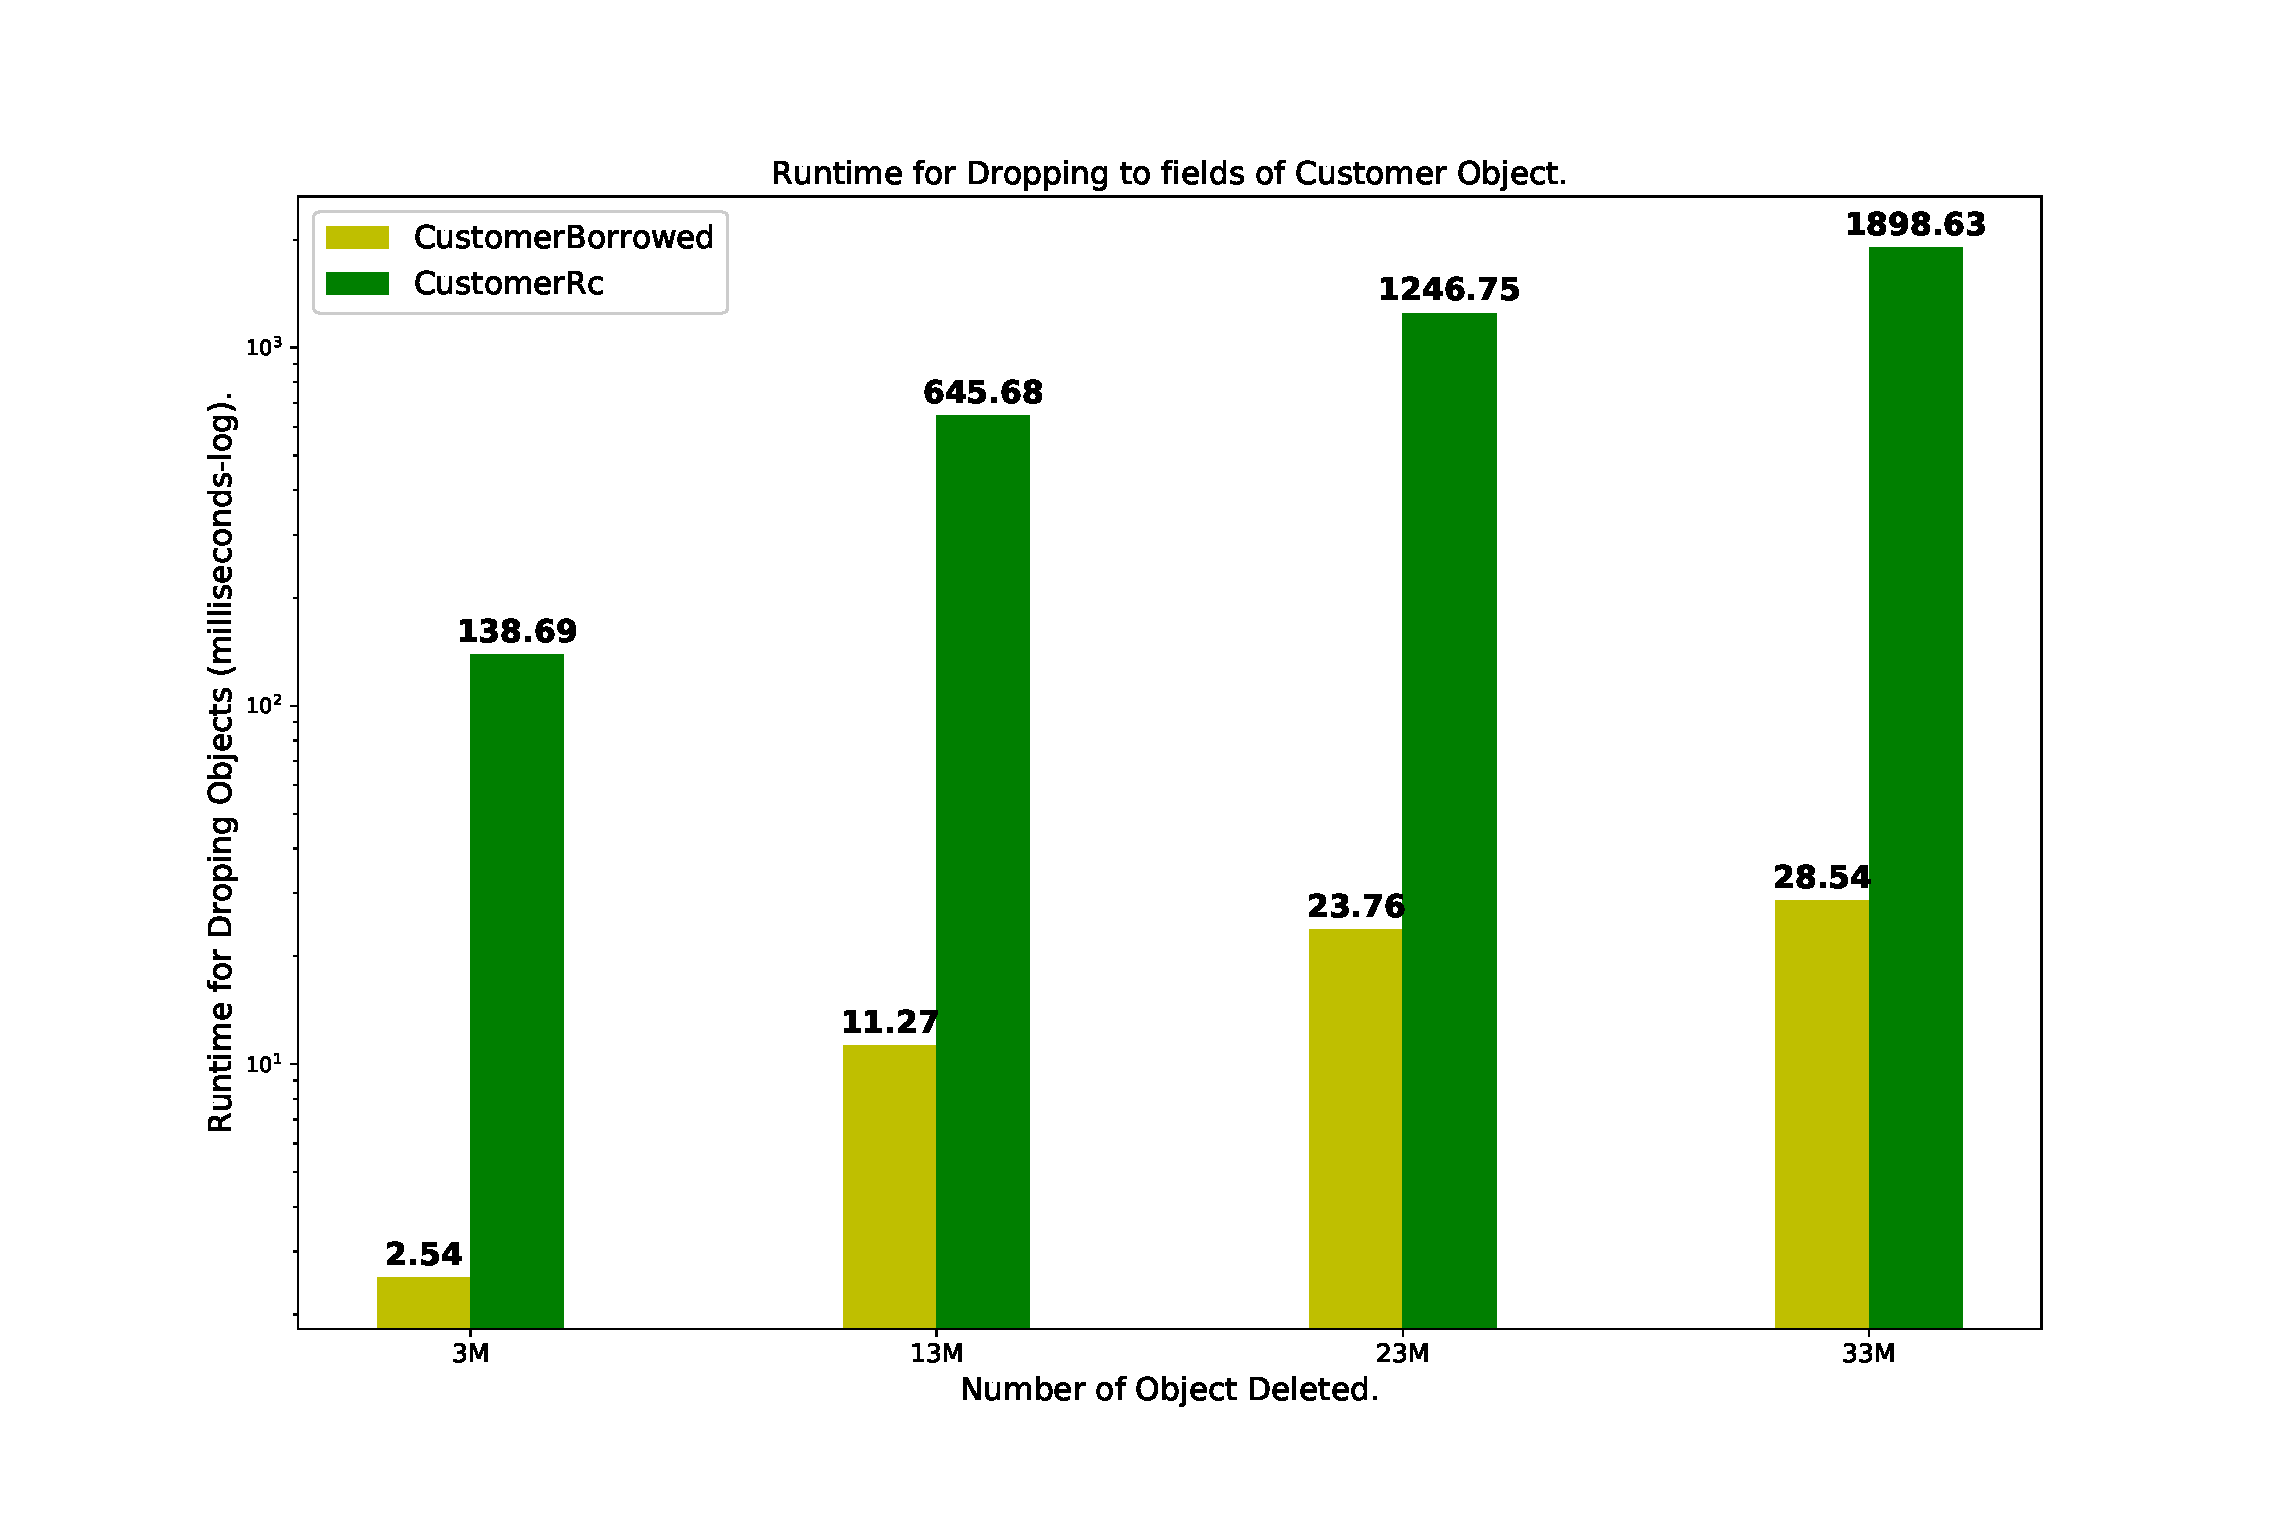
\includegraphics[width=0.8\textwidth]{images/rust_droptime_borring_rc.eps}
                \captionsetup{labelformat=empty}
                % \caption{\textbf{}}
        \end{center}
    \end{figure}
    Dropping Reference Counting is about \blueb{60 times slower} than normal reference.
\end{frame}

%%%%%%%%%%%%%%%%%%%%%%%%%%%%%%%%%%%%%%%%%%%%
%%%%%%%%%%%%%%%%%%%%%%%%%%%%%%%%%%%%%%%%%%%%

\begin{frame}[fragile]{Experiment 3: Merge-sort}

    Question
    \begin{itemize}
        \item How much does sharing set of data with Atomic Reference Counting slowdown merge-sort algorithms?
    \end{itemize}

    Evaluation
    \begin{itemize}
        \item Share \blueb{vector} of complex objects
        \item \blueb{Atomic Reference Counting (Arc)} vs \blueb{normal reference}
        \item Measure \blueb{runtime of merge-sort algorithms}
    \end{itemize}

\end{frame}

%%%%%%%%%%%%%%%%%%%%%%%%%%%%%%%%%%%%%%%%%%%%
%%%%%%%%%%%%%%%%%%%%%%%%%%%%%%%%%%%%%%%%%%%%


\begin{frame}[fragile]{Experiment 3: Merge-sort}

    \begin{figure}[hp]
        \centering
        \begin{center}
                \includegraphics[width=0.8\textwidth]{images/rust_merge_sort.eps}
                \captionsetup{labelformat=empty}
                % \caption{\textbf{}}
        \end{center}
    \end{figure}
    \vspace{-.1 cm}
    Algorithms with Arc are about \blueb{21\%  slower.}
\end{frame}

%%%%%%%%%%%%%%%%%%%%%%%%%%%%%%%%%%%%%%%%%%%%
%%%%%%%%%%%%%%%%%%%%%%%%%%%%%%%%%%%%%%%%%%%%

\begin{frame}[fragile]{Experiment 4: Tree-aggregate}

    Question
    \begin{itemize}
        \item How much are runtime differences between sharing elements of data with Arc and deep-copying elements of data?
    \end{itemize}

    Evaluation
    \begin{itemize}
        \item Share \blueb{elements} of complex object
        \item \blueb{Atomic Reference Counting (ARC)} vs \blueb{Deep copy}
        \item Measure \blueb{runtime of Tree-aggregate algorithms}
    \end{itemize}

\end{frame}

%%%%%%%%%%%%%%%%%%%%%%%%%%%%%%%%%%%%%%%%%%%%
%%%%%%%%%%%%%%%%%%%%%%%%%%%%%%%%%%%%%%%%%%%%

\begin{frame}[fragile]{Experiment 4: Tree-aggregate}

    \begin{figure}[hp]
        \centering
        \begin{center}
                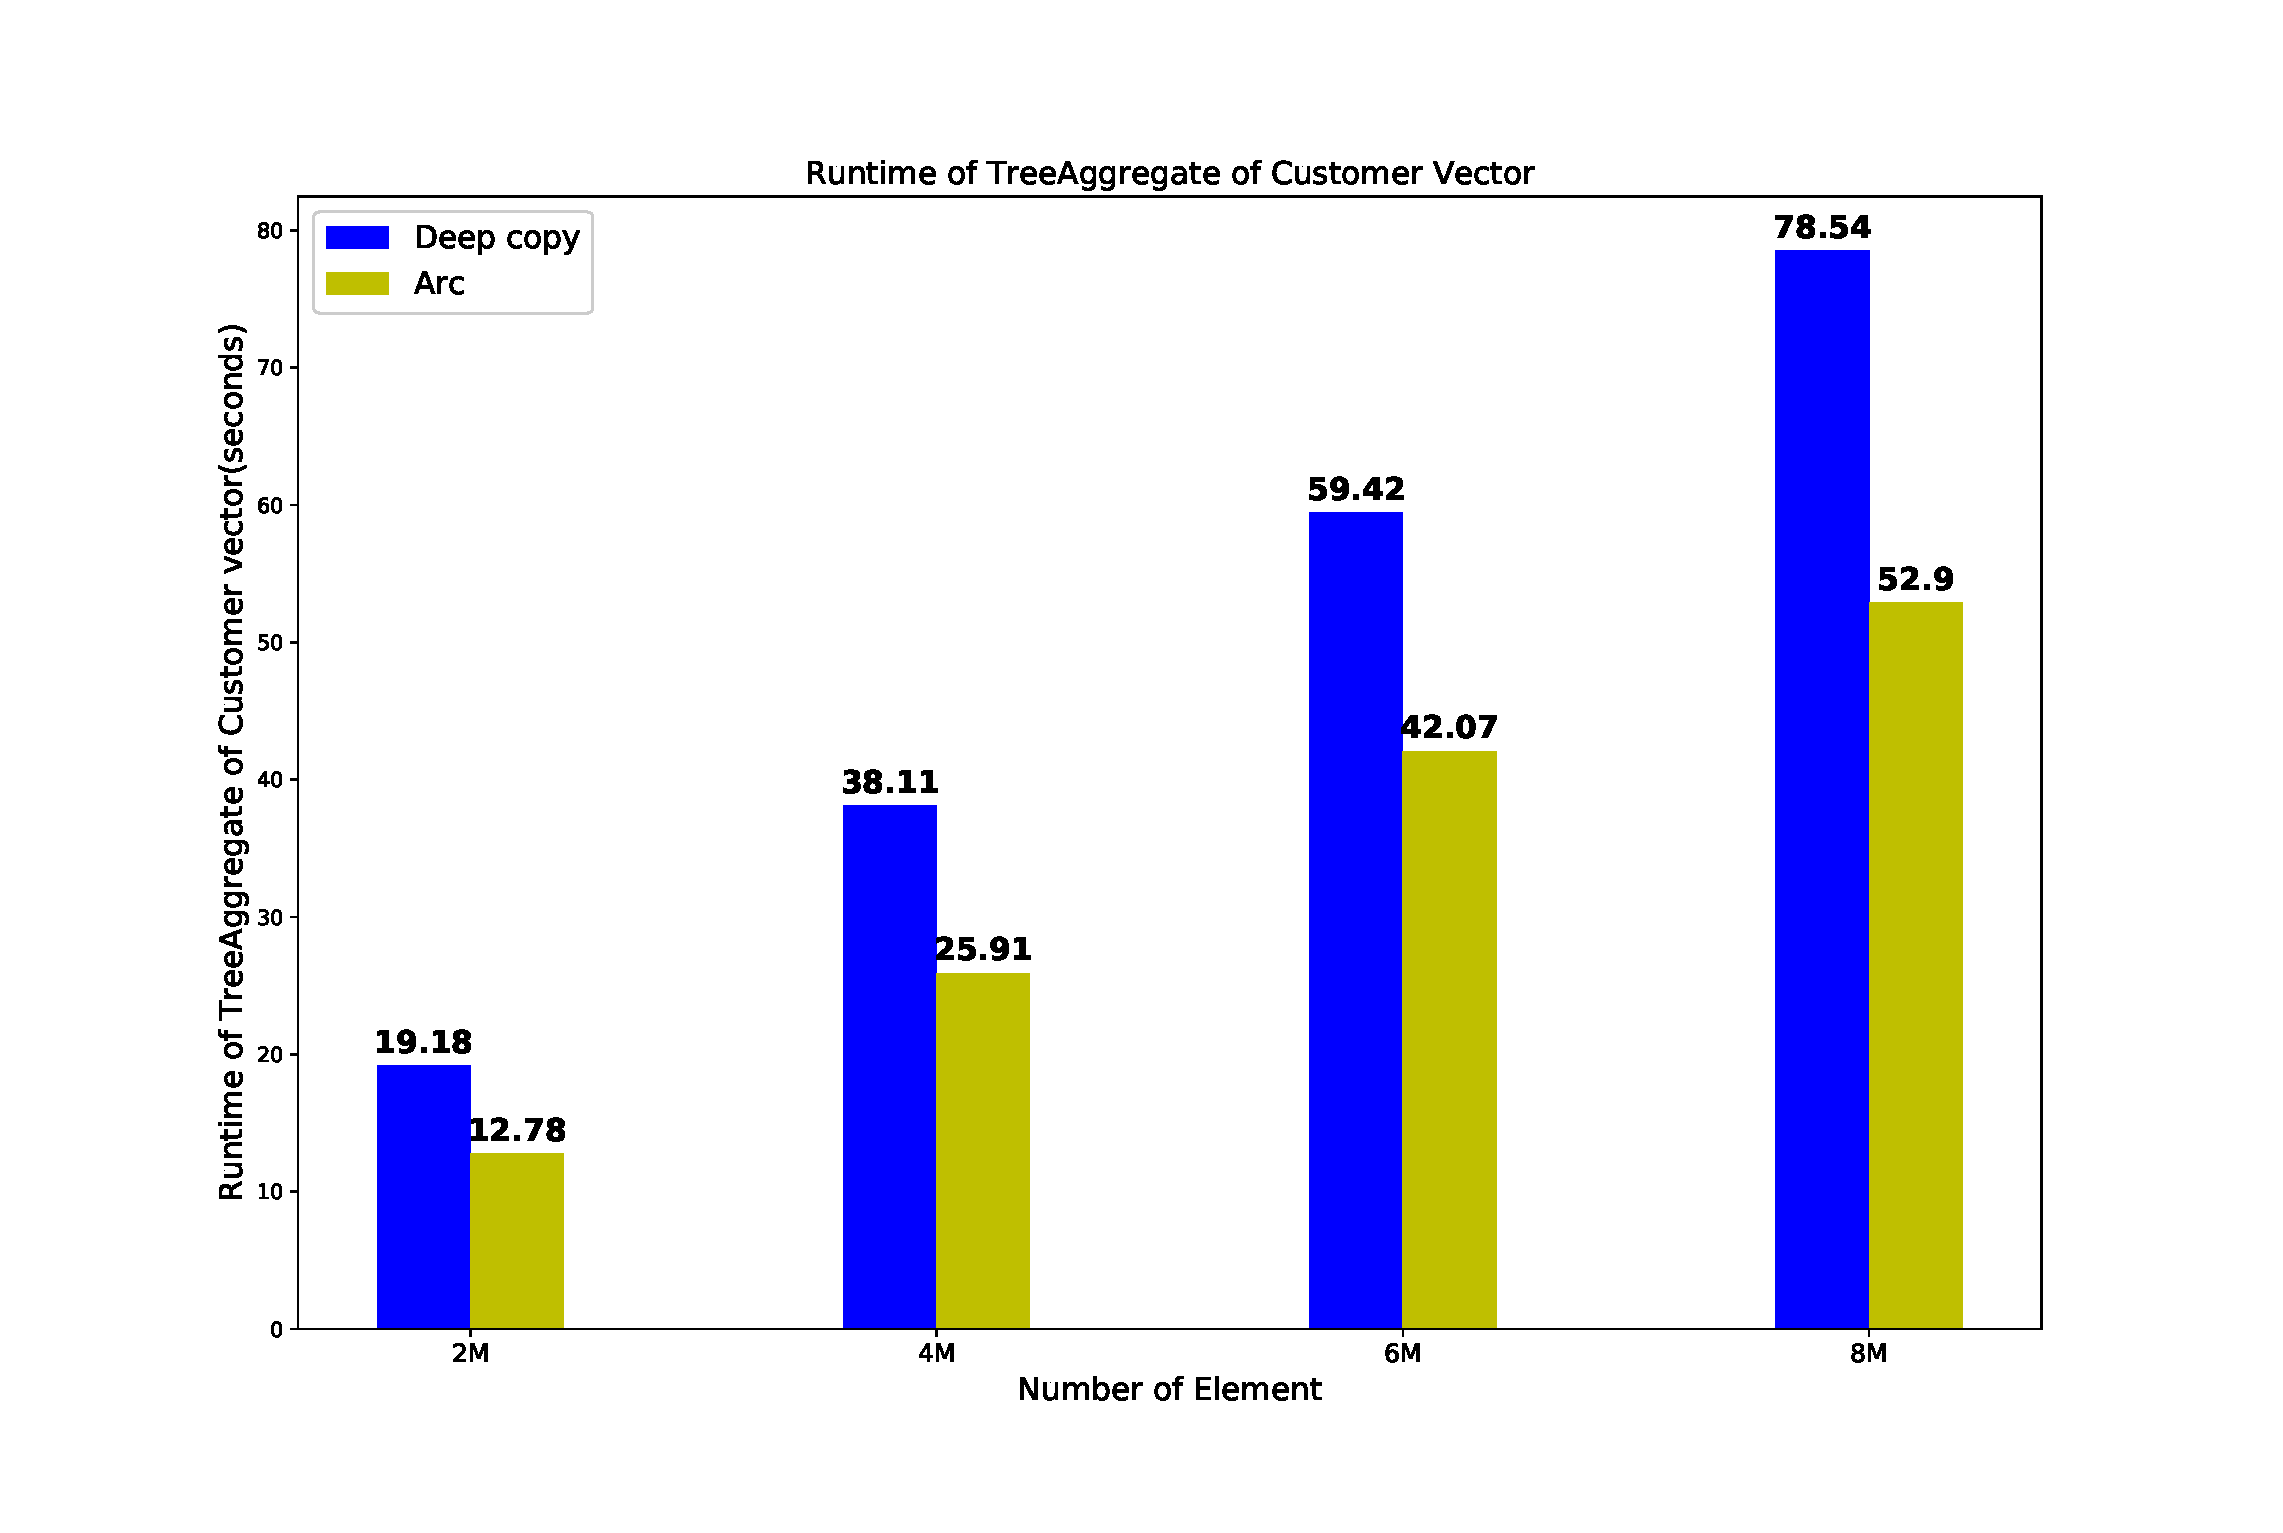
\includegraphics[width=0.8\textwidth]{images/rust_tree_aggregate.eps}
                \captionsetup{labelformat=empty}
                % \caption{\textbf{}}
        \end{center}
    \end{figure}
    \vspace{-.1 cm}
    Algorithms with deep-copy are from \blueb{40 to 50\% slower.}
\end{frame}

%%%%%%%%%%%%%%%%%%%%%%%%%%%%%%%%%%%%%%%%%%%%
%%%%%%%%%%%%%%%%%%%%%%%%%%%%%%%%%%%%%%%%%%%%

\begin{frame}[fragile]{Experiment 5: K-Nearest-Neighbors (KNN)}

    Question
    \begin{itemize}
        \item What are better memory management strategies for common Machine Learning Algorithms?
    \end{itemize}

    Evaluation
    \begin{itemize}
        \item Document classification on Wikipedia page dataset
        \item Preprocessing phase: calculating \blueb{Term-frequencies (Tfs)}
        \item String manipulation
        \item \blueb{Atomic Reference Counting (Arc)} vs \blueb{Deep copy}
        \item \blueb{Frequency of memory de/allocation}
        \begin{itemize}
            \item batch number
            \item strategy
            \begin{itemize}
                \item 1: keep intermediate objects in memory until owner is changed
                \item 2: remove intermediate objects as soon as it is not needed
            \end{itemize}
        \end{itemize}
        \item Measure runtime of \blueb{preprocessing time of KNN algorithms}
    \end{itemize}
\end{frame}

%%%%%%%%%%%%%%%%%%%%%%%%%%%%%%%%%%%%%%%%%%%%
%%%%%%%%%%%%%%%%%%%%%%%%%%%%%%%%%%%%%%%%%%%%

\begin{frame}[fragile]{Experiment 5: K-Nearest-Neighbors}

    \begin{figure}[hp]
        \centering
        \begin{center}
                \includegraphics[width=0.8\textwidth]{images/preprocessing.eps}
                \captionsetup{labelformat=empty}
                % \caption{\textbf{}}
        \end{center}
    \end{figure}
    \begin{itemize}
        \item Algorithms with \blueb{Arc} are \blueb{at most 38 \% slower} than deep-copy.
        \item Algorithms with \blueb{strategy 2} are \blueb{at most 85 \% slower} than strategy 1.
        \item Algorithms with \blueb{3 batches} are \blueb{at most 40 \% slower} than 2 batches.
    \end{itemize}
\end{frame}

%%%%%%%%%%%%%%%%%%%%%%%%%%%%%%%%%%%%%%%%%%%%
%%%%%%%%%%%%%%%%%%%%%%%%%%%%%%%%%%%%%%%%%%%%

\begin{frame}[fragile]{Conclusion}
    \begin{itemize}
        \item Use normal reference rather than Reference Counting whenever it is possible.
        \item Trade-off between \blueb{runtime performance} and \blueb{lifetime tracking}.
        \item \blueb{Avoid using Arc} when we can use reference.
        \item Use Arc instead of deep-copy, when \blueb{complexity of objects is large}.
        \item Use deep-copy, when \blueb{complexity of objects is small}, like String.
    \end{itemize}
\end{frame}


% \section{Some Terminology}

% \begin{frame}[fragile, t ]{Convex Function}
% A function $f(x)$ is defined to be convex when
% \begin{align*}
% \forall x_1, x_2 \in X, \forall t \in [0,1]: f(t x_1 + (1 - t) x_2) \leq t f(x_1) + (1 - t) f(x_2)
% \end{align*}
% \vspace{-.5cm}

% \begin{minipage}{.49\linewidth}
% \begin{figure}[hp]
% \centering
% \begin{center}
%     	\includegraphics[width=1\textwidth]{images/convexFunction.pdf}
%     	\captionsetup{labelformat=empty}
%     	\caption{\textbf{Convex Function}}
% \end{center}
% \end{figure}
% \end{minipage}
% \pause
% \begin{minipage}{.49\linewidth}
% \begin{figure}[hp]
% \centering
% \begin{center}
%     	\includegraphics[width=1\textwidth]{images/concaveFunction.pdf}
%     	\captionsetup{labelformat=empty}
%     	\caption{\textbf{Concave Function}}
% \end{center}
% \end{figure}
% \end{minipage}
% \begin{itemize}
%   \item For maximum of a Concave function, we calculate minimum of $-f(x)$
% \end{itemize}

% \end{frame}


% %%%%%%%%%%%%%%%%%%%%%%%%%%%%%%%%%%%%%%%%%%%%
% %%%%%%%%%%%%%%%%%%%%%%%%%%%%%%%%%%%%%%%%%%%%

% \begin{frame}{None Convex Functions - Global and }

% \begin{center}
%     	\includegraphics[width=0.8\textwidth]{images/GlobalMin.png}
% \scalebox{.5}{Image from Book:   Ian Goodfellow, Yoshua Bengio, Aaron Courville - Deep Learning - The MIT Press (2016)}

% \end{center}

% \end{frame}




% %
% %%%%%%%%%%%%%%%%%%%%%%%%%%%%%%%%%%%%%%%%%%%%%
% %%%%%%%%%%%%%%%%%%%%%%%%%%%%%%%%%%%%%%%%%%%%%
% %\section{Example - Doing Regression \\ Computation can be expensive}
% %\begin{frame}[fragile, t ]{Example - Doing Regression}
% %We have a set of training data like \\
% %
% %\begin{itemize}
% %\item Data Matrix of  \blueb{$X \in  \mathbb{R}^{n \times d}$},  with Labels \blueb{$Y \in  \mathbb{R}^{n  \times 1}$}
% %    \item Linear Regression Model :
% %   \end{itemize}
% %\large
% %\begin{center}
% %$y = \theta_0+ \theta_1 x_1 + \theta_2 x_2 + ... + \theta_d x_d + e $ \\
% %\end{center}
% %\pause
% %\text{The same in matrix form: }
% %\begin{center}
% %\blueb{
% %$Y_{n \times 1 } = X_{n \times d}   \Theta_{d \times 1 }  + e_{n \times 1} $
% %}\normalsize
% %
% %
% %Find \blueb{ $ \Theta \in \mathbb{R}^{d \times 1}$} to minimize
% %
% %
% %\large
% %$MSE(\Theta) = \frac{1}{N} e^T e$
% %\end{center}
% %\normalsize
% %
% %
% %\pause
% %
% %
% %Finding exact  solution:
% %
% %\begin{itemize}
% %  \item This function is a \brownb{convex function}.
% %  \item Take the derivative and set it to zero
% %
% %\Large
% %\blueb{
% %   $\Theta = (X^T X )^{-1} X^T Y$
% %}
% %\end{itemize}
% %
% %
% %\end{frame}
% %
% %
% %
% %
% %
% %%%%%%%%%%%%%%%%%%%%%%%%%%%%%%%%%%%%%%%%%%%%%
% %%%%%%%%%%%%%%%%%%%%%%%%%%%%%%%%%%%%%%%%%%%%%
% %\begin{frame}[fragile, t ]{Doing Regression - Computation Costs}
% %
% % In computing exact solution:
% %
% %\begin{center}
% %\blueb{
% %\Large
% %  $\Theta = (X^T X )^{-1} X^T Y$
% %}
% %\end{center}
% %
% %\begin{itemize}
% %  \item We know that \textbf{$n$ number of data rows can be large}
% %  \item  \greenb{If dimension $d$ is small}, then
% % \blueb{$X^T X \in   \mathbb{R}^{n \times d} $}  and \blueb{$X^T Y \in  \mathbb{R}^{d \times 1}$}
% %
% %are in good size to compute in parallel on a single machine.
% %
% %\end{itemize}
% %
% %\pause
% %
% %\greenb{Nice!} This can be  one line code in R Program\\
% %\blueb{ solve(t(X) \%*\% X) \%*\% t(X) \%*\% y}.
% %
% %\pause
% %\vspace{0.5cm}
% %\redb{But what if the  \textbf{dimension $d$ is large}? }
% %
% %We would need a large size of memory for computing matrix operations
% %(Matrix-Matrix, Matrix-Vector).
% %
% %\end{frame}

% %%%%%%%%%%%%%%%%%%%%%%%%%%%%%%%%%%%%%%%%%%%%
% %%%%%%%%%%%%%%%%%%%%%%%%%%%%%%%%%%%%%%%%%%%%
% \section{Gradient Descent}

% \begin{frame}[fragile, t]{Gradient Descent}
% Most widely used optimization framework for  - at least -  \textbf{"Big Data'' science }is \textbf{gradient descent}.


% What is the idea?

% \begin{itemize}
%     \item \textcolor{blue}{Gradient Descent is an iterative algorithm}
%     \item Goal: \blueb{ choose $\theta^*$ to minimize cost
%     function $L(\theta) $ }
%     \item \textcolor{blue}{Start from an initial guess and try to incrementally improve current solution}
%     \item \textcolor{blue}{At iteration step $\theta^{(iter)}$ is the current guess for $\theta^*$}

% \end{itemize}

% \vspace{-.3 cm}

% \begin{center}
%     \includegraphics[width=0.5\textwidth]{images/gd1.pdf}
% \end{center}

% \end{frame}


% %%%%%%%%%%%%%%%%%%%%%%%%%%%%%%%%%%%%%%%%%%%%
% %%%%%%%%%%%%%%%%%%%%%%%%%%%%%%%%%%%%%%%%%%%%

% \begin{frame}[fragile,t]{What is a Gradient?}

% \blueb{Gradient} is the multi-dimensional analog to a \blueb{derivative}

% \begin{itemize}
%     \item $\nabla L(\theta)$ is a vector-valued function
%     \item It is a vector whose \blueb{$i$th} entry is \blueb{$i$th} partial derivative evaluated at
%     \blueb{$\theta_i$}
% \end{itemize}

% \centering

% \large
% \blueb{
% $\nabla L(\theta) =
% \begin{bmatrix}
% 	\frac{\partial L(\theta)}{\partial \theta_0}  \\
% 	\frac{\partial L(\theta)}{\partial \theta_1} \\
%    	. \\
%    	. \\
%    	. \\
%    	\frac{\partial L(\theta)}{\partial \theta_d} \\
% \end{bmatrix}
% $
%   }

% \vspace{0.5cm}

% \begin{itemize}
%     \item \textbf{Negative of gradient indicates direction of steepest descent}
%     \item We use the gradient to find out the direction of steepest descent in multidimensional space.
% \end{itemize}


% \end{frame}



% %%%%%%%%%%%%%%%%%%%%%%%%%%%%%%%%%%%%%%%%%%%%
% %%%%%%%%%%%%%%%%%%%%%%%%%%%%%%%%%%%%%%%%%%%%

% \begin{frame}[fragile, t]{Gradient Descent - Basic algorithm}

% \begin{center}
% \begin{minipage}{.55\linewidth} % find the minimal value to enclose the code

% \begin{algorithmic}

% \State $\theta^{(iter)} \gets \text{an initial guess for } \theta^*$
% \State $iter \gets 1 $
% \Repeat
%     \State $\theta^{(iter + 1 )} \gets \theta^{(iter)} - \lambda \nabla
%     L(\theta^{(iter)})$
%     \State $iter \gets iter+1$
% \Until{$(\text{Stop Condition})$ }

% \end{algorithmic}

% \end{minipage}
% \end{center}


% \vspace{0.5cm}

% \begin{itemize}
%     \item \textcolor{blue}{Here $\lambda$ is the \redb{"learning rate"}} and controls speed of convergence

%     \item \textcolor{blue}{$\nabla L(\theta_{iter})$ is the \redb{gradient} of L evaluated at iteration "$iter$" with parameter of $\theta_{iter}$ }

% 	\item Stop conditions can be different
% \end{itemize}


% \end{frame}




% %%%%%%%%%%%%%%%%%%%%%%%%%%%%%%%%%%%%%%%%%%%%
% %%%%%%%%%%%%%%%%%%%%%%%%%%%%%%%%%%%%%%%%%%%%

% \begin{frame}[fragile]{When to Stop?}
% \vspace{-.5cm}


% \begin{center}
% \begin{minipage}{.55\linewidth} % find the minimal value to enclose the code

% \begin{algorithmic}
% \State $\theta^{(iter)} \gets \text{an initial guess for } \theta^*$
% \State $iter \gets 1 $
% \Repeat
%     \State $\theta^{(iter +1 )} \gets \theta^{(iter)} - \lambda \nabla
%     L(\theta^{(iter)})$

%     \State $iter \gets iter+1$
% \Until{$(\text{Stop Condition})$ }
% \end{algorithmic}

% \end{minipage}

% \noindent\rule{6cm}{0.4pt}

% \end{center}

% % \noindent\makebox[\linewidth]{\rule{\paperwidth}{0.4pt}}



% Stop condition can be different, for example:

% \begin{itemize}
% 	\item \blueb{Maximum number of iteration is reached}    $(iter < MaxIteration)$
%     \item \blueb{Gradient $\nabla L(\theta^{(iter)}) $ or parameters are not
%     changing }$  (||\theta^{(iter+1)} - \theta^{(iter)}|| < precisionValue ) $
%     \item\blueb{Cost is not decreasing}  $ (||L(\theta^{(iter+1)}) -
%     L(\theta^{(iter)} ) || < precisionValue ) $
%     \item \blueb{Combination of the above}
% \end{itemize}

% Mostly we stop it based on number of iterations\\
%  \textit{(Early stop to avoid  "Over-fitting")}.
% \end{frame}



% %%%%%%%%%%%%%%%%%%%%%%%%%%%%%%%%%%%%%%%%%%%%
% %%%%%%%%%%%%%%%%%%%%%%%%%%%%%%%%%%%%%%%%%%%%

% % \begin{frame}[fragile, t]{Example}
% %
% % Returning to linear regression . . .
% %
% % \begin{itemize}
% %     \item \textcolor{blue}{Want a line to fit points $\langle 118, 122, 145,
% %     149, 186 \rangle$ }
% %     \item \textcolor{blue}{At time ticks $t$ in $\langle1, 2, 3, 4, 5\rangle$}
% %     \item \textcolor{blue}{Prediction $f(t|c,m) = c+m \times t$}
% %     \item \textcolor{blue}{Loss function $L(c,m) = \sum_i(f(t_i |c,m ) -x_i)^2$}
% % \end{itemize}
% %
% %
% % \end{frame}

% %%%%%%%%%%%%%%%%%%%%%%%%%%%%%%%%%%%%%%%%%%%%
% %%%%%%%%%%%%%%%%%%%%%%%%%%%%%%%%%%%%%%%%%%%%
% %
% % \begin{frame}[t]{Example}
% % Returning to linear regression . . .
% %
% % \begin{itemize}
% %     \item \textcolor{blue}{Prediction $f(t|c,m) = c+m \times t$}
% %     \item \textcolor{blue}{Loss function is Mean Squared Error $L(c,m) =  \frac{1}{N} \sum_i(f(t_i |c,m ) -x_i)^2$}
% %
% % \end{itemize}
% %
% % First we deal with c and m:
% %
% % \begin{align*}
% %     {\partial F } \over  {\partial c}  &= \Large \sum_i 2 (f(t_i |c, m ) - x_i) \\
% %     {\partial F } \over  {\partial m}  &= \Large \sum_i 2 t_i (f(t_i |c, m ) - x_i) \\
% %     So\ that \\
% %     \nabla L(c,m)  &=\langle \Large  \sum_i 2 (f(t_i |c, m ) - x_i)  , \Large \sum_i 2 t_i (f(t_i |c, m ) - x_i) \rangle\\
% % \end{align*}
% %
% % We can divide the loss by 2 to make derivative calculations simpler.
% %
% % \end{frame}

% % %%%%%%%%%%%%%%%%%%%%%%%%%%%%%%%%%%%%%%%%%%%%
% % %%%%%%%%%%%%%%%%%%%%%%%%%%%%%%%%%%%%%%%%%%%%
% %
% % \begin{frame}[t]{Grad Descent and Big Data}
% %
% % Gradient of the following form is very common
% %
% % \large{
% % \begin{align*}
% %     \nabla L(c,m)  &=\langle \Large  \sum_i 2 (f(t_i |c, m ) - x_i)  , \Large \sum_i 2 t_i (f(t_i |c, m ) - x_i) \rangle\\
% % \end{align*}
% % }
% %
% % \Large{
% % Why is this so good for "Big Data"? MapReduce?}
% %
% %
% %
% % \end{frame}


% %%%%%%%%%%%%%%%%%%%%%%%%%%%%%%%%%%%%%%%%%%%%
% %%%%%%%%%%%%%%%%%%%%%%%%%%%%%%%%%%%%%%%%%%%%

% \begin{frame}[fragile, t]{Example - Back to Multiple Linear Regression Model}
% \vspace{-.2cm}
% \begin{align*}
% y = \theta_0+ \theta_1 x_1 +  \dots + \theta_d x_d \\
% MSE=L(\Theta) =  \frac{1}{2N} \sum_{i=1}^{n} (y^{i} - (\theta_0+ \theta_1 x_1 + ... + \theta_d
% x_d))^2
% \end{align*}

% \redb{How to compute the gradient with many dimensions? }
% \pause

% Compute partial derivatives
% \large
% \blueb{
% \begin{align*}
% \frac{\partial L }{\partial  \theta_1} & =  \frac{-1}{N} \sum_{i=1}^{n} x^{(i)}_1 (y^{(i)} - (\theta_0 + \theta_1 x^{(i)}_1+ \dots  + \theta_d x^{(i)}_d)) \\
% \frac{\partial L}{\partial  \theta_2} & =  \frac{-1}{N} \sum_{i=1}^{n} x^{(i)}_2 (y^{(i)} - (\theta_0 + \theta_1 x^{(i)}_1+ \dots  + \theta_d x^{(i)}_d)) \\
% \dots  & \\
% \end{align*}
% }
% \normalsize
% Compute components of the gradients \textbf{(map operation)} and then sum them up and update weights in the next iteration \textbf{(reduce operation)}

% \end{frame}


% %%%%%%%%%%%%%%%%%%%%%%%%%%%%%%%%%%%%%%%%%%%%
% %%%%%%%%%%%%%%%%%%%%%%%%%%%%%%%%%%%%%%%%%%%%


% \begin{frame}[fragile, t]{Map Reduce Implementation}

% \begin{lstlisting}
% // initialize parameters
% iter= 0
% learningRate= 0.01
% numIteration= 400
% theta = np.zeros(noParameters)

% while (iter < maxNumIteration):
%   reduceData = myData.map(
%           // Calculate the gradients
%       )
%       .reduce(
%           // update model parameters
%           // lambda theta :  - learningRate * theta
%       )
%   iter = iter+1

% \end{lstlisting}

% In Spark you can  \blueb{reduceByKey() }or better \blueb{aggregateByKey()}


% \end{frame}




% %%%%%%%%%%%%%%%%%%%%%%%%%%%%%%%%%%%%%%%%%%%%
% %%%%%%%%%%%%%%%%%%%%%%%%%%%%%%%%%%%%%%%%%%%%

% \section{Learning Rate is Super Important}

% %%%%%%%%%%%%%%%%%%%%%%%%%%%%%%%%%%%%%%%%%%%%
% %%%%%%%%%%%%%%%%%%%%%%%%%%%%%%%%%%%%%%%%%%%%
% \begin{frame}[fragile,t]{Gradient Descent - learning rate too Small (Slow convergence)}
% The learning rate is Super important.

% \textcolor{blue}{Too small: many, many passes through the data to converge}

% \begin{center}
%     	\includegraphics[width=0.5\textwidth]{images/slow.pdf}
% \end{center}



% \end{frame}


% %%%%%%%%%%%%%%%%%%%%%%%%%%%%%%%%%%%%%%%%%%%%
% %%%%%%%%%%%%%%%%%%%%%%%%%%%%%%%%%%%%%%%%%%%%
% \begin{frame}[fragile,t]{Gradient Descent}

%    \textcolor{blue}{Too large: Jumping around}

% \begin{center}
%     \includegraphics[width=0.5\textwidth]{images/fast.pdf}
% \end{center}

% \end{frame}




% %%%%%%%%%%%%%%%%%%%%%%%%%%%%%%%%%%%%%%%%%%%%
% %%%%%%%%%%%%%%%%%%%%%%%%%%%%%%%%%%%%%%%%%%%%
% \begin{frame}[fragile,t]{Gradient Descent - Oscillations}

%    \textcolor{blue}{Too large: oscillate into oblivion}

% \begin{center}
%     \includegraphics[width=0.6\textwidth]{images/oscillations.pdf}
% \end{center}

% \end{frame}

% %%%%%%%%%%%%%%%%%%%%%%%%%%%%%%%%%%%%%%%%%%%%
% %%%%%%%%%%%%%%%%%%%%%%%%%%%%%%%%%%%%%%%%%%%%

% \begin{frame}{Choose Learning Rate - Line Search }

% Best option (in terms of results) but \redb{most expensive}:

% \begin{itemize}
%     \item Solve another mini-optimization problem
%     \item Select $\lambda$ so as to minimize $L(\theta^{(iter)})$
%     \item It's a 1-dimensional optimization problem!
%     \item Called a line search
% \end{itemize}

% \end{frame}


% %%%%%%%%%%%%%%%%%%%%%%%%%%%%%%%%%%%%%%%%%%%%
% %%%%%%%%%%%%%%%%%%%%%%%%%%%%%%%%%%%%%%%%%%%%

% \begin{frame}[fragile, t]{Line Search}

% \begin{algorithmic}
% \State $l \gets 0$
% \State $h \gets 999999 $

% \While{$  ( h - l >\epsilon )$ }
%     \State $ h' \gets l + {{{1} \over {c}}(h-l)} $
%     \State $ l' \gets h - {{{1} \over {c}}(h-l)} $

%     \State $goodness_h \gets L(\theta^{(i)} - h' \nabla L(\theta^{(iter)}))$
%     \State $goodness_l \gets L(\theta^{(i)} - l' \nabla L(\theta^{(iter)}))$

%     \If{ $( goodness_h <  goodness_l)$}
%         \State $l \gets l'$
%     \Else
%         \State $h \gets h'$
%     \EndIf


% \EndWhile

% \end{algorithmic}
% \large


% \textcolor{red}{"Golden Section Search"} $ c = {{{1} \over {2}} (1 + \sqrt{5})} = 1.618 $


% \end{frame}



% %%%%%%%%%%%%%%%%%%%%%%%%%%%%%%%%%%%%%%%%%%%%
% %%%%%%%%%%%%%%%%%%%%%%%%%%%%%%%%%%%%%%%%%%%%

% \begin{frame}[fragile, t]{Other Ways To Choose Learning Rate - "Bold Driver"}

% Line search is very costly!

% One other standard method is \textcolor{red}{"Bold Driver"}

% \begin{itemize}
%     \item \textcolor{blue}{Make a very conservative initial guess for $\lambda$  } \\
%    \textcolor{blue}{At each iteration, compute the cost $L(\Theta^{(iter)} )$ }

%     \item \textcolor{blue}{Better than last time?
%      \\
%      $ \lambda \gets   1.05 \times \lambda $}
%       \\
%      \brownb{If cost decreases, increase learning rate}
% 		\\
%     \item \textcolor{blue}{Worse than last time? \\
%     $ \lambda \gets  0.5 \times \lambda$}
%       \\
% 	\brownb{If cost increases, decrease rate}
% \end{itemize}

% \textbf{This would be then just one evaluation of loss function per iteration!}
% \end{frame}


% %%%%%%%%%%%%%%%%%%%%%%%%%%%%%%%%%%%%%%%%%%%%
% %%%%%%%%%%%%%%%%%%%%%%%%%%%%%%%%%%%%%%%%%%%%

% \begin{frame}{Cost Monitoring - "Bold Driver" vs. Constant Learning Rates}

% \normalsize
% \begin{center}
%     	\includegraphics[width=0.75\textwidth]{images/graph02.pdf}
% \end{center}

% \vspace{-.7cm}

% Text Classification with Logistic regression (20k Dimensions Term Frequencies) .


% \begin{itemize}
%   \item Horizontal axis is number of iterations
%   \item Vertical axis shows value of negative log-likelihood
% \end{itemize}

% \end{frame}

% %%%%%%%%%%%%%%%%%%%%%%%%%%%%%%%%%%%%%%%%%%%%
% %%%%%%%%%%%%%%%%%%%%%%%%%%%%%%%%%%%%%%%%%%%%

% \begin{frame}{Text Classification with Logistic regression - Different Learning Rate}

% \vspace{-.4cm}
% \begin{center}
%     	\includegraphics[width=0.9\textwidth]{images/DifferentLearningRate.pdf}
% \end{center}

% \vspace{-.5cm}

% The same Text Classification with 20k Dimensions,  term frequencies of words

% \end{frame}





% %%%%%%%%%%%%%%%%%%%%%%%%%%%%%%%%%%%%%%%%%%%%
% %%%%%%%%%%%%%%%%%%%%%%%%%%%%%%%%%%%%%%%%%%%%

% \begin{frame}{Example  - Very Large Learning Rate}

% \vspace{-.4cm}
% \begin{center}
%     	\includegraphics[width=0.7\textwidth]{images/VeryLargeAndSmallLearningRate.pdf}
% \end{center}

% \vspace{-.5cm}

% The same Text classification with 20k Dimensions,  term frequencies of words


% \begin{itemize}
% 	\item Very small learning rate of 0.001
% 	\item Very Large learning rate
% 	\item Good working learning rate.
% \end{itemize}

% \end{frame}




% %%%%%%%%%%%%%%%%%%%%%%%%%%%%%%%%%%%%%%%%%%%%
% %%%%%%%%%%%%%%%%%%%%%%%%%%%%%%%%%%%%%%%%%%%%

% \begin{frame}{Text Classification with Logistic regression - Large Learning Rate}

% \vspace{-.4cm}
% \begin{center}
%     	\includegraphics[width=0.7\textwidth]{images/graph01.pdf}
% \end{center}

% \vspace{-.5cm}

% 20k Dimensions,  term frequencies of words

% \begin{itemize}
% 	\item Very small learning rate of 0.001
% 	\item Large learning rate
% 	\item Good working learning rate.
% \end{itemize}

% \end{frame}




% %%%%%%%%%%%%%%%%%%%%%%%%%%%%%%%%%%%%%%%%%%%%
% %%%%%%%%%%%%%%%%%%%%%%%%%%%%%%%%%%%%%%%%%%%%
% \section{Variations of Gradient Descent}

% \begin{frame}{Variations of Gradient Descent}

% Depending on Size of data that we use in each iteration:

% \begin{itemize}
%     \item \brownb{Full Batch Gradient Descent} (Using the whole data set (size n))
%     \item \brownb{Stochastic Gradient Descent (SGD)}  (Using one sample per iteration (size 1))
%     \item \blueb{Mini Batch Gradient Descent} (Using a mini batch of data (size $m < n$))
% \end{itemize}

% Some times people refer to SGD  as  mini batch.
% \end{frame}


% %%%%%%%%%%%%%%%%%%%%%%%%%%%%%%%%%%%%%%%%%%%%
% %%%%%%%%%%%%%%%%%%%%%%%%%%%%%%%%%%%%%%%%%%%%

% \begin{frame}{Stochastic Gradient Descent}
% Calculate the gradient of a single sample and update parameters in
%     each iterations

% \begin{itemize}
%     \item Pick up samples for update by \textbf{sequential read (pass over the data} - do not
%     take random sample from a big data set in each iterations  - computationally expensive)


%      \item It is noisy and sometimes  will do lots of iterations
%     \item Do not be afraid of \textbf{non-convex functions}, SGD can help to \blueb{get out of local minimums}.

%     \item It is a widely applied approach

%     \item SGD is often faster in producing good results.

% \end{itemize}
% \end{frame}



% %%%%%%%%%%%%%%%%%%%%%%%%%%%%%%%%%%%%%%%%%%%%
% %%%%%%%%%%%%%%%%%%%%%%%%%%%%%%%%%%%%%%%%%%%%

% \begin{frame}{Mini-Batch Gradient Descent}

% Something between Stochastic and Full-batch

% \begin{itemize}
%     \item Pick up mini batch samples for update by sequential pass over the data and use it to update
%     \item Batch gradient descent has  better convergence rates than stochastic
%     gradient descent in theory.
%     \item But we may not to pursue to converge fast (presumably results in overfitting)

%     \item Depending on size, can help to  out of local minimums.
% \end{itemize}


% Implementation Tips:
% \begin{itemize}
%     \item Use mini-batch data size of 64, 256, 512, ... (power of 2))
%     \item Make sure that mini-batch data fits in CPU/GPU memory
% \end{itemize}


% \end{frame}


% %%%%%%%%%%%%%%%%%%%%%%%%%%%%%%%%%%%%%%%%%%%%
% %%%%%%%%%%%%%%%%%%%%%%%%%%%%%%%%%%%%%%%%%%%%

% \begin{frame}{Implementation Tips:}


% \begin{itemize}
%     \item \blueb{Monitor the costs in each iteration to check if it decreases.}
%     \item \textbf{Map} to calculate gradients, \textbf{Reduce} to update the weights
%     \item Use vectorization of computations (run bulk operations, e.g., use numpy inside Spark RDDs or Spark Dataframes)
% \end{itemize}

% \end{frame}


% %%%%%%%%%%%%%%%%%%%%%%%%%%%%%%%%%%%%%%%%%%%%
% %%%%%%%%%%%%%%%%%%%%%%%%%%%%%%%%%%%%%%%%%%%%

% \begin{frame}{Issues of Gradient Descent}


% \begin{itemize}
%     \item You can find local min/max and not Global
%     \item There is no grantee that you can find the global minimum
%     \item All depends on Starting point, Step-Size and Function type.
% \end{itemize}

% The main problem is : \\
% \redb{Oscillate into oblivion}

% \end{frame}





% %%%%%%%%%%%%%%%%%%%%%%%%%%%%%%%%%%%%%%%%%%%%
% %%%%%%%%%%%%%%%%%%%%%%%%%%%%%%%%%%%%%%%%%%%%

% \begin{frame}[fragile,t]{Gradient Descent with Momentum }

% \textbf{A momentum} is a moving average of our gradients.


% \centering
% \Large
% \blueb{
% \begin{align*}
% V^{(iter)} = &  \beta   V^{iter - 1} +  (1 - \beta ) \nabla L(W, X, y) \\
% W^{(iter+1)} = & W^{(iter)} - \lambda   V^{(iter)}
% \end{align*}
% }

% \begin{itemize}
% 	\item $\beta $ is a positive number

% 	\item $\lambda $ is learning rate

% 	\item $ L(W, X, y)$ is cost function

% 	\item $W$ is vector of weights (model parameters)
% \end{itemize}

% \end{frame}







% %%%%%%%%%%%%%%%%%%%%%%%%%%%%%%%%%%%%%%%%%%%%
% %%%%%%%%%%%%%%%%%%%%%%%%%%%%%%%%%%%%%%%%%%%%

% \begin{frame}{Further methods }



% \begin{itemize}

%   	\item Adaptive gradient algorithm (AdaGrad)
%     \item Root Mean Square Propagation (RMSProp)
%     \item \brownb{Adaptive Moment Estimation (Adam)}
%     \item ...
% \end{itemize}

% \end{frame}





% %%%%%%%%%%%%%%%%%%%%%%%%%%%%%%%%%%%%%%%%%%%%
% %%%%%%%%%%%%%%%%%%%%%%%%%%%%%%%%%%%%%%%%%%%%

% \begin{frame}{ADAM: A METHOD FOR STOCHASTIC OPTIMIZATION }


% \begin{center}
%     	\includegraphics[width=0.9\textwidth]{images/Adam.png}
% \end{center}

% Logistic regression training negative log likelihood on MNIST images and IMDB movie
% reviews with 10,000 bag-of-words (BoW) feature vectors.

% (Image from Kingma et. al 2017)
% \end{frame}







% %%%%%%%%%%%%%%%%%%%%%%%%%%%%%%%%%%%%%%%%%%%%
% %%%%%%%%%%%%%%%%%%%%%%%%%%%%%%%%%%%%%%%%%%%%

% \begin{frame}{Summary}

% \brownb{Gradient Descent is a great optimization algorithm}

% \begin{itemize}
%     \item Gradient descent is a \textbf{first-order} iterative optimization algorithm
%     and is easy to use.
%     \item Widely applicable in many different machine learning methods
%     \item But convergence can be slow
% \end{itemize}




% \end{frame}


% %%%%%%%%%%%%%%%%%%%%%%%%%%%%%%%%%%%%%%%%%%%%
% %%%%%%%%%%%%%%%%%%%%%%%%%%%%%%%%%%%%%%%%%%%%
% %
% \begin{frame}[t]{Some of the related publications }

% \footnotesize
% \begin{itemize}
%   	\item  Diederik P. Kingma, Jimmy Ba (2015). \textit{Adam: A Method for Stochastic Optimization.} In proceeding of ICLR 2015: San Diego, CA, USA

%   	\item John Duchi, Elad Hazan, and Yoram Singer (2011). \textit{Adaptive
%   	Subgradient Methods for Online Learning and Stochastic Optimization.} Journal of Machine Learning Research, 12:2121–2159, 2011.
%   	\item Timothy Dozat (2016). \textit{Incorporating Nesterov Momentum into
%   	Adam.} ICLR  	Workshop, (1):2013–2016, 2016.

%     \item Bottou, Léon (1998). \textit{Online Algorithms and Stochastic Approximations.} Online Learning and Neural Networks. Cambridge University Press. ISBN 978-0-521-65263-6

%     \item Bottou, Léon (2010). \textit{Large-scale machine learning with SGD.} Proceedings of COMPSTAT’2010. Physica-Verlag HD, 2010. 177-186.

%     \item Bottou, Léon (2012). \textit{SGD tricks. Neural Networks: Tricks of the Trade.} Springer Berlin Heidelberg, 2012. 421-436.

% \end{itemize}

% \end{frame}



% %%%%%%%%%%%%%%%%%%%%%%%%%%%%%%%%%%%%%%%%%%%%
% %%%%%%%%%%%%%%%%%%%%%%%%%%%%%%%%%%%%%%%%%%%%
% \section{Extra Slides}


% %%%%%%%%%%%%%%%%%%%%%%%%%%%%%%%%%%%%%%%%%%%%
% %%%%%%%%%%%%%%%%%%%%%%%%%%%%%%%%%%%%%%%%%%%%
% \section{Example - Doing Regression \\ Computation can be expensive}

% \begin{frame}[fragile, t ]{Example - Doing Regression}
% We have a set of training data like \\

% \begin{itemize}
% \item Data Matrix of  \blueb{$X \in  \mathbb{R}^{n \times d}$},  with Labels \blueb{$Y \in  \mathbb{R}^{n  \times 1}$}
%     \item Linear Regression Model :
% \large
% \begin{align*}
% y = & \theta_0+ \theta_1 x_1 + \theta_2 x_2 + ... + \theta_d x_d + e \\
% \text{The same in matrix form:   } Y_{n \times 1 } = & X_{n \times d}   \Theta_{d \times 1 }  + e_{n \times 1}
% \end{align*}
%  \normalsize

%     \pause
%     \item We are looking for a vector of parameters (set of weights)

%     \blueb{$\Theta \in \mathbb{R}^{d \times 1}$} to minimize
% \begin{center}
% \large
% $MSE=L(\Theta) = \frac{1}{N} e^T e =  \frac{1}{N}  (y^T y - 2 \Theta^T X^T  y + \Theta^T X^T  X \Theta )$
%  % \frac{1}{N} \sum_{i=1}^{n} (y_i - (\theta_0+ \theta_1 x_1 + ... + \theta_d x_d))^2$
% \end{center}
% \normalsize
% \end{itemize}
% \pause

% Finding exact  solution:

% \begin{itemize}
%   \item This function is a \brownb{convex function}.
%   \item Take the derivative and set it to zero

% \Large
% \blueb{
%   $ \frac{d }{d  \Theta}  L(\Theta)= -2 X^T (Y - X \Theta)  = 0 $
% }
% \end{itemize}

%  We set the above to zero and will get
% \Large
% \begin{center}
% \blueb{$\Theta = (X^T X )^{-1} X^T Y$}
% \end{center}

% \end{frame}










\end{document}
